% === LaTeX Figure Includes for UAV-Embodied-IQA ===
% Updated 2026-07-22 — added fig_vlm_corr, fig_dataset_stats, TABLE_1_database_stats
% Copy snippets into the paper as needed.

% ── Figure: Cognitive Score Distribution Across 36 Distortion Types ──
% Equivalent to Embodied-IQA Figure 4 (subjective)
\begin{figure}[t]
    \centering
    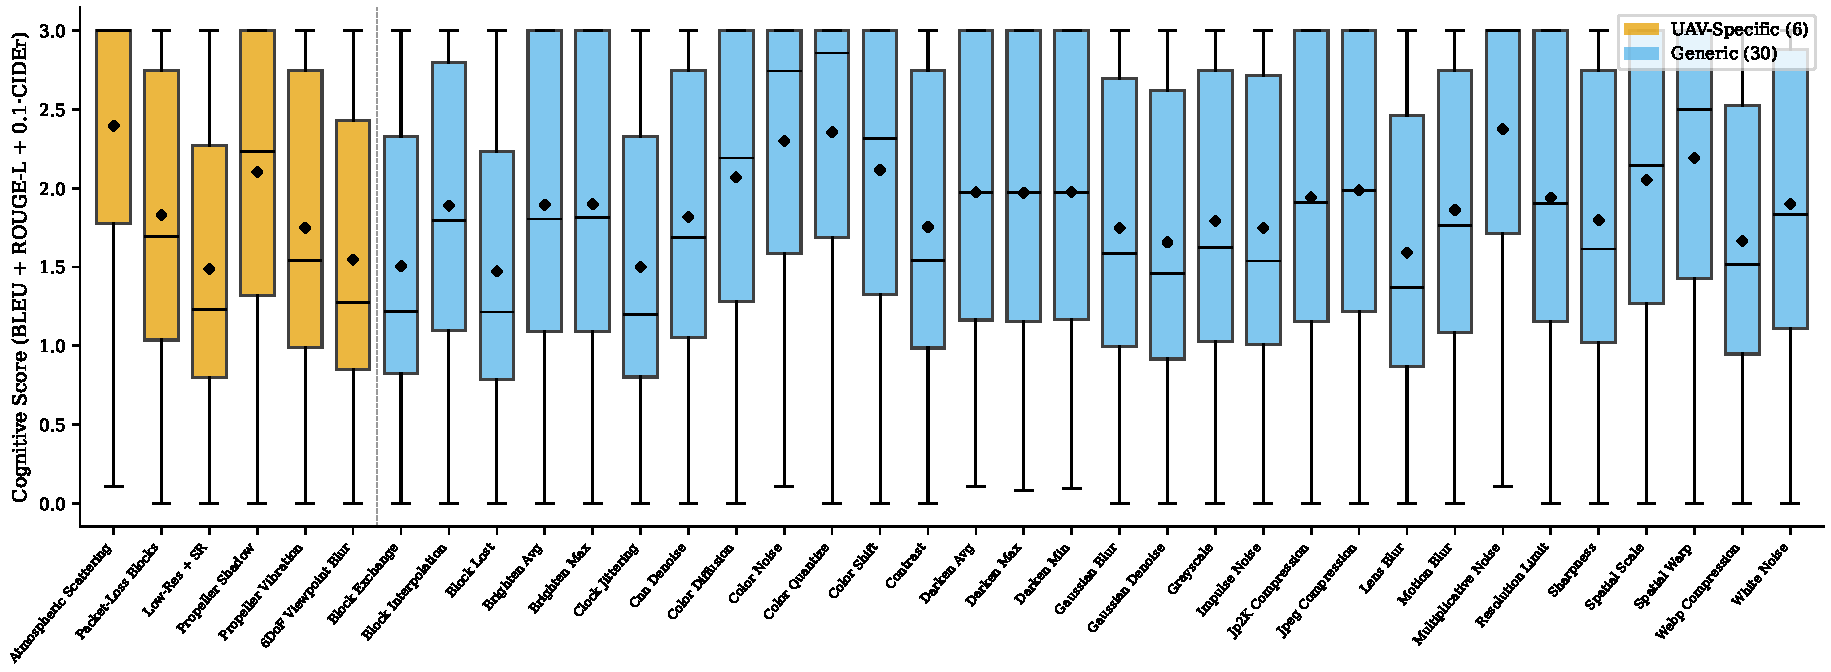
\includegraphics[width=\textwidth]{figures/fig1_distribution.pdf}
    \caption{Distribution of VLM cognitive scores across all 36 distortion types.
    Boxes show median and interquartile range; diamonds indicate means.
    UAV-specific distortions (orange, left of dashed line) exhibit distinct cognitive
    score distributions compared to generic distortions (blue).
    Cognitive score = BLEU + ROUGE-L + 0.1·CIDEr, averaged across all VQA task prompts.}
    \label{fig:distribution}
\end{figure}

% ── Figure: UAV vs Generic Distortion Comparison ──
\begin{figure}[t]
    \centering
    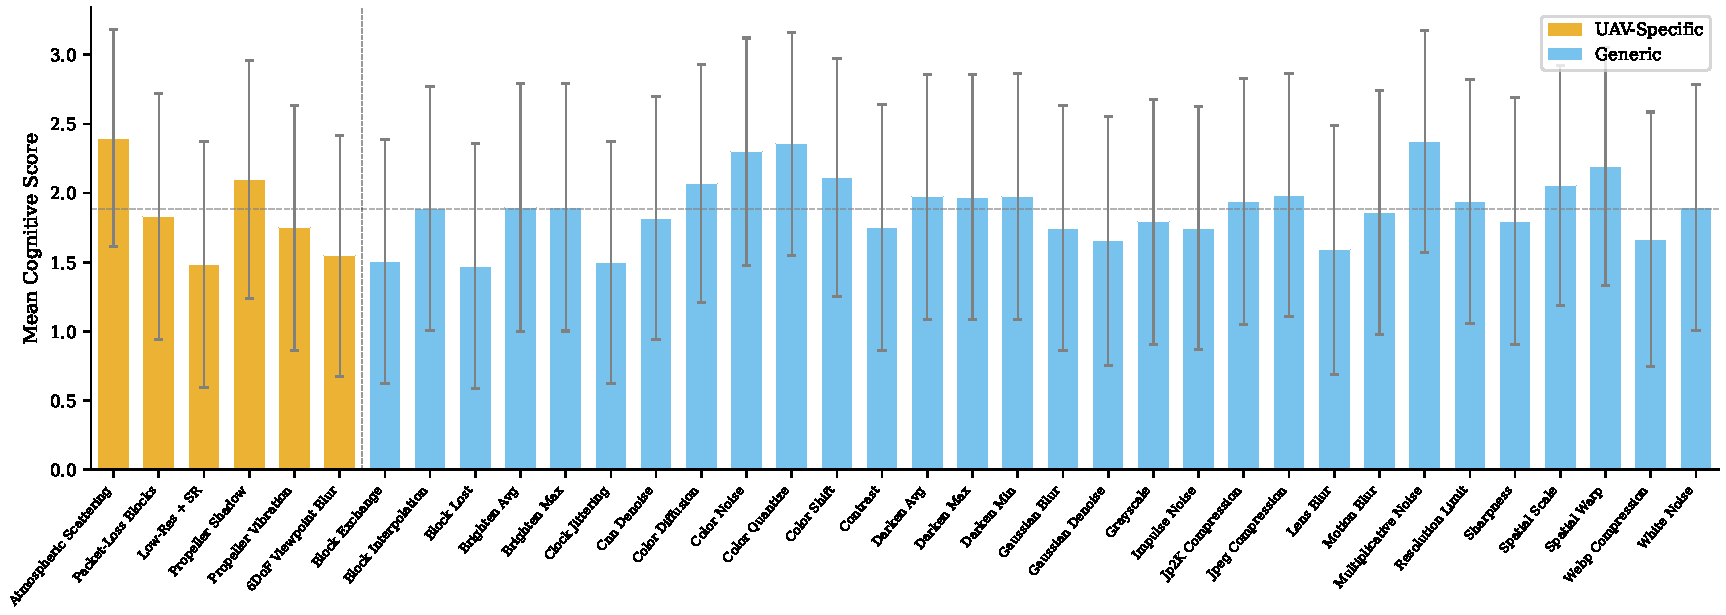
\includegraphics[width=\textwidth]{figures/fig2_uav_vs_generic.pdf}
    \caption{Mean cognitive score per distortion type, grouped by UAV-specific (orange)
    vs. generic (blue). Error bars show ±1 standard deviation. The dashed horizontal
    line marks the grand mean across all distortions. UAV distortions span a wide
    range: propeller shadow and atmospheric scattering produce relatively mild
    cognitive degradation, while low-res+SR artifacts and 6DoF viewpoint blur
    cause severe performance drops.}
    \label{fig:uav_vs_generic}
\end{figure}

% ── Figure: 3-D Score Breakdown per Distortion Category ──
\begin{figure}[t]
    \centering
    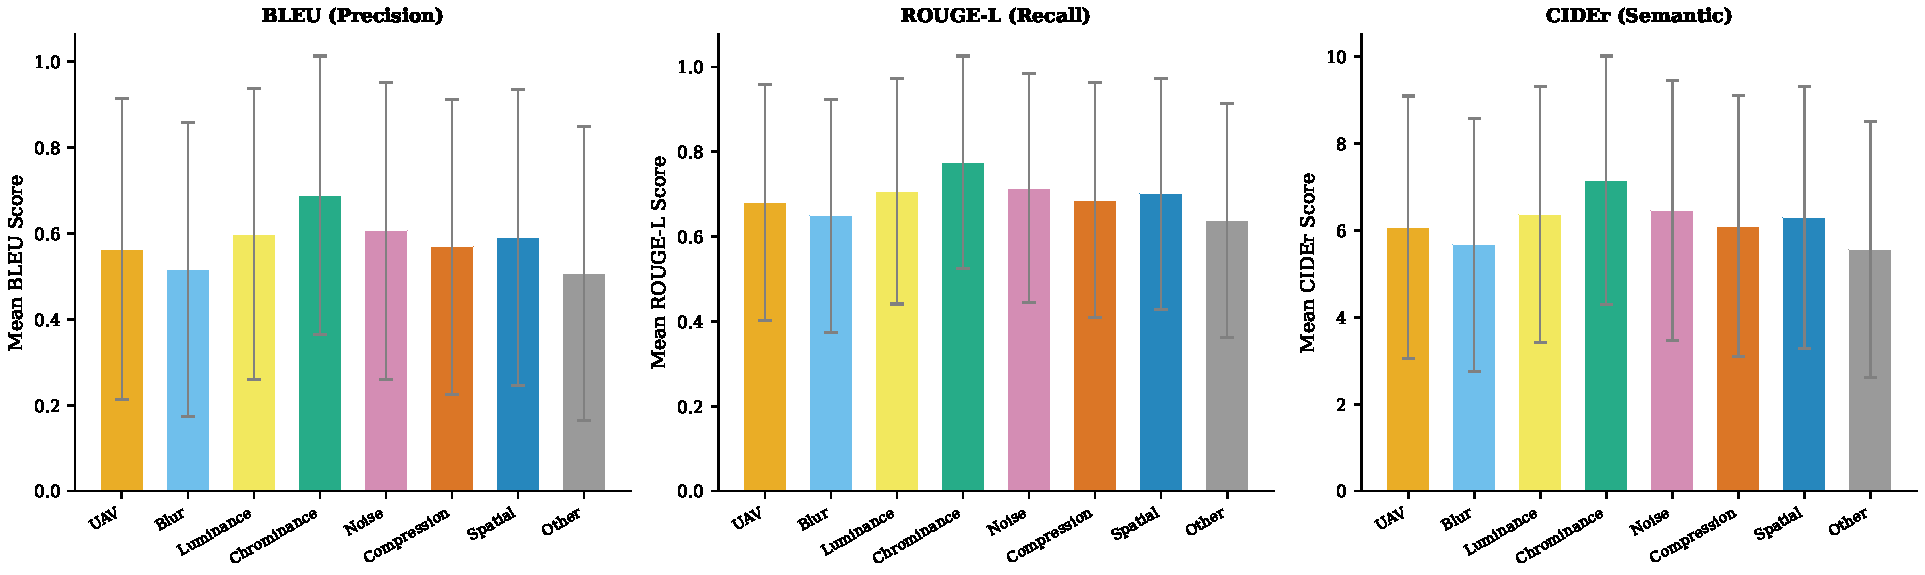
\includegraphics[width=\textwidth]{figures/fig3_three_dimensions.pdf}
    \caption{Three-dimensional cognitive score decomposition across distortion
    categories. BLEU (left) captures token-level precision loss; ROUGE-L (center)
    captures recall of critical information; CIDEr (right) captures semantic-level
    degradation. UAV distortions show a distinctive profile: moderate BLEU/ROUGE-L
    degradation but relatively preserved CIDEr, indicating UAV-specific distortions
    primarily affect surface-level text fidelity rather than semantic understanding.}
    \label{fig:three_dimensions}
\end{figure}

% ── Figure: JND-based Sensitivity Classification ──
% Equivalent to Embodied-IQA Figure 7 (JND)
\begin{figure}[t]
    \centering
    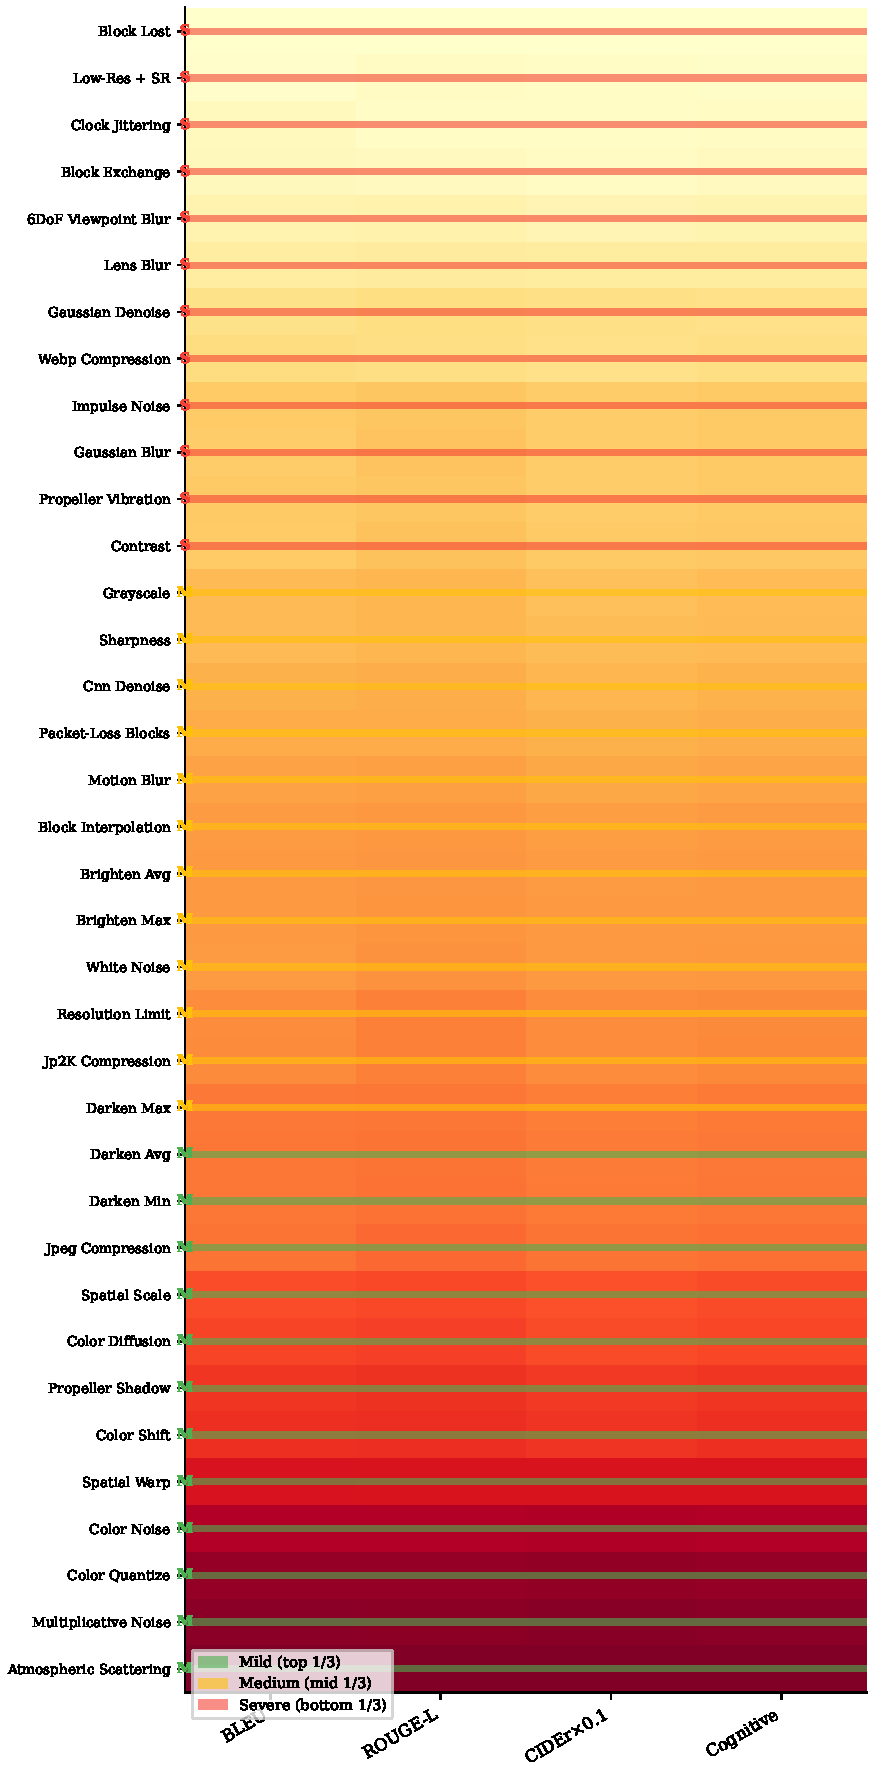
\includegraphics[width=0.65\textwidth]{figures/fig4_jnd_sensitivity.pdf}
    \caption{Just-Noticeable-Difference (JND) sensitivity classification for all 36
    distortion types. Distortions are sorted by mean cognitive score into three tiers:
    Mild (green, top third), Medium (yellow, middle third), and Severe (red, bottom
    third). Colored bars on the left indicate JND tier. Heatmap columns show normalized
    contributions of BLEU, ROUGE-L, CIDEr×0.1, and the composite cognitive score.
    UAV distortions span all three JND tiers, confirming they produce a wide spectrum
    of cognitive degradation severity.}
    \label{fig:jnd_sensitivity}
\end{figure}

% ── Figure: Per-Intensity Degradation Curves ──
\begin{figure}[t]
    \centering
    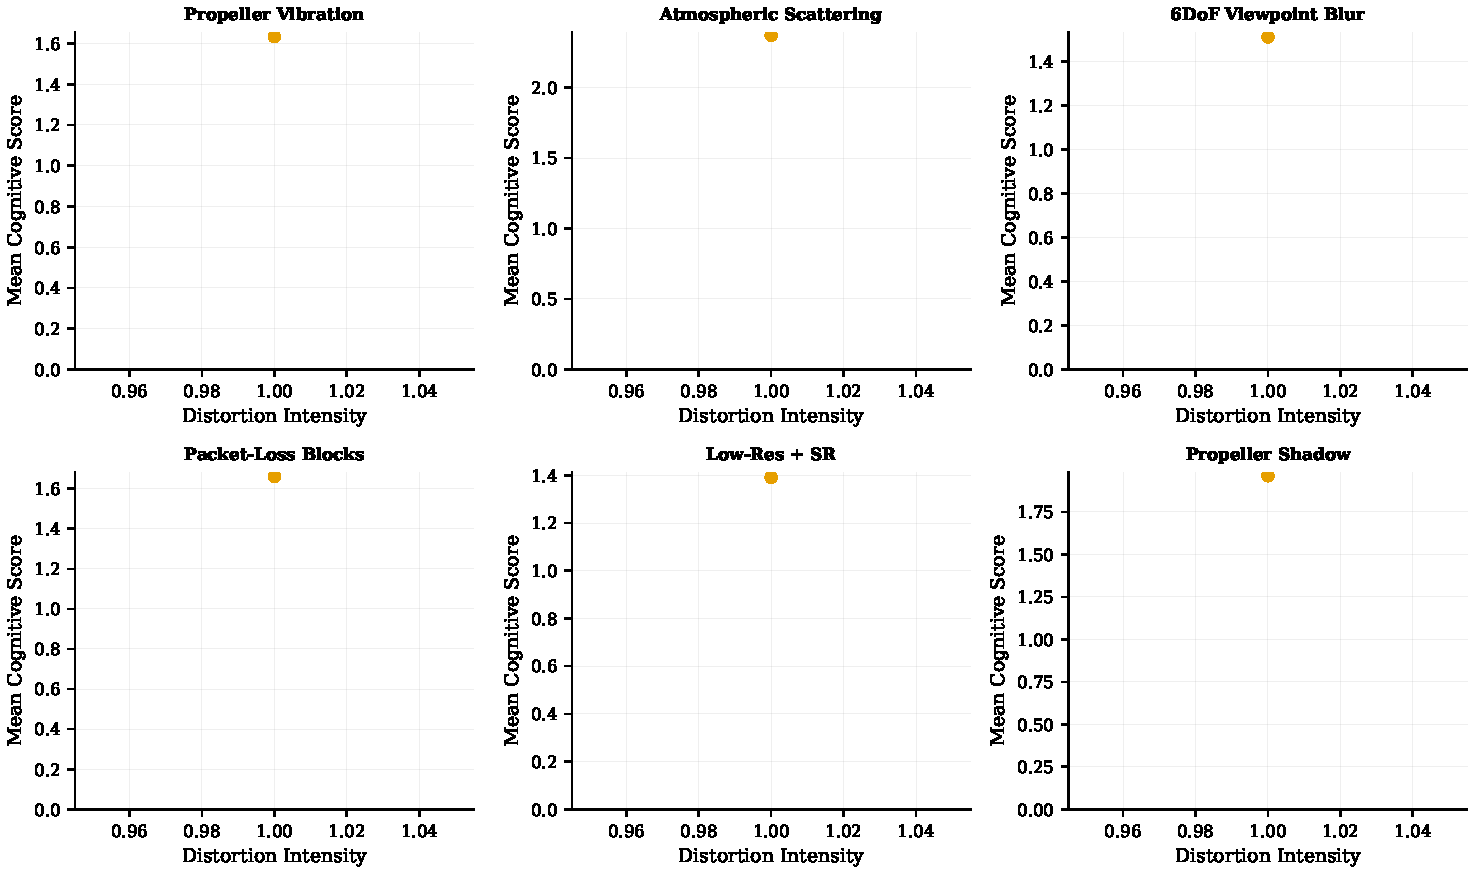
\includegraphics[width=\textwidth]{figures/fig5_intensity_curves.pdf}
    \caption{Cognitive score as a function of distortion intensity for the 6
    UAV-specific distortion types. Most UAV distortions show approximately monotonic
    cognitive degradation with increasing intensity. Propeller shadow and atmospheric
    scattering show relatively flat curves (robust to intensity changes), while
    low-res+SR and 6DoF viewpoint blur show steeper degradation slopes.}
    \label{fig:intensity_curves}
\end{figure}

% ── Figure: Source Comparison (Simulation vs Real) ──
\begin{figure}[t]
    \centering
    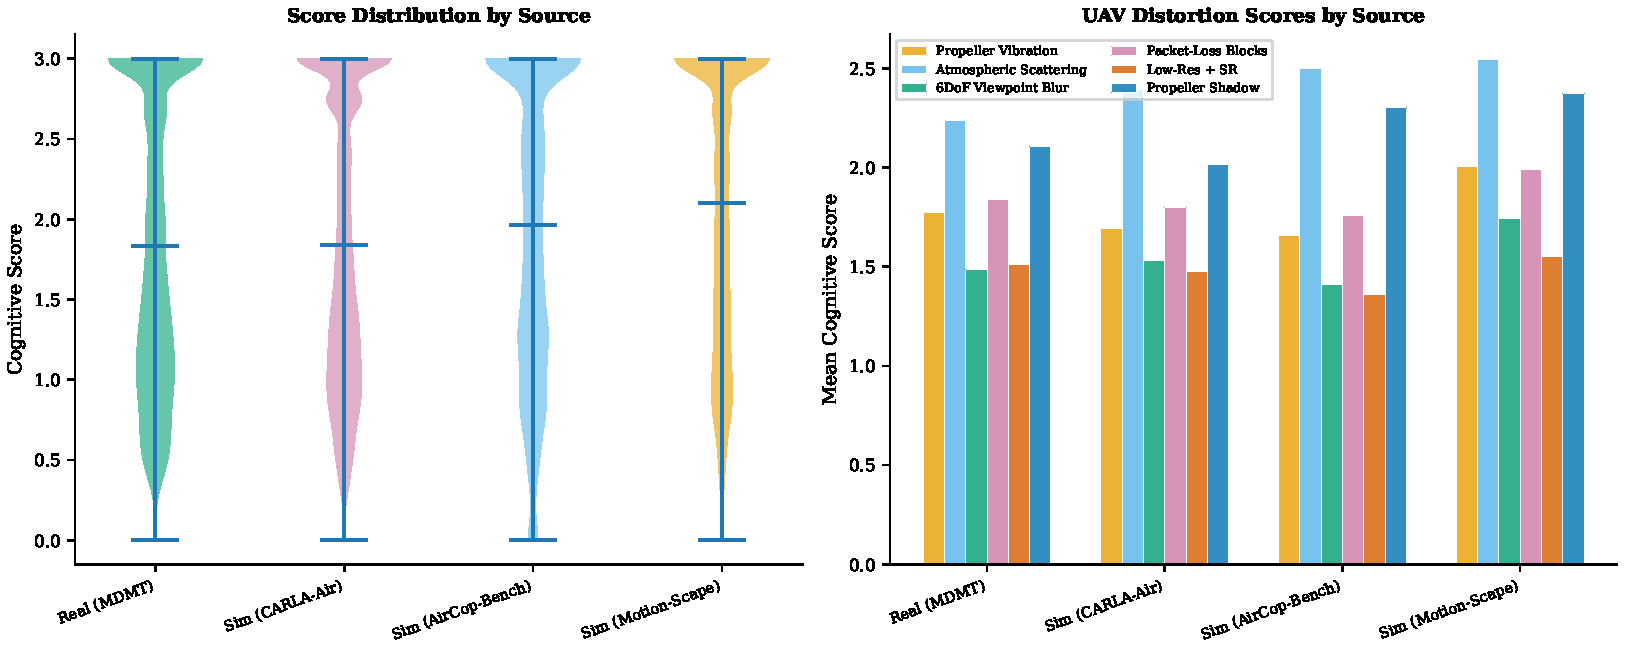
\includegraphics[width=\textwidth]{figures/fig6_source_comparison.pdf}
    \caption{Cognitive score comparison across image sources. (Left) Violin plots
    showing score distributions for Sim3 (CARLA-Air), Sim5 (AirCopBench),
    Sim6 (MotionScape), and Real2 (MDMT real-world). Real-world images from MDMT
    consistently yield higher cognitive scores, suggesting VLMs handle natural
    scenes more robustly than rendered simulation imagery under distortion.
    (Right) Per-UAV-distortion score breakdown by source, revealing that the
    synthetic-to-real score gap varies by distortion type.}
    \label{fig:source_comparison}
\end{figure}

% ── Figure: Inter-VLM SRCC Correlation Matrix ──
% Supports §3.3 annotation reliability argument (see also Embodied-IQA §3.2)
\begin{figure}[t]
    \centering
    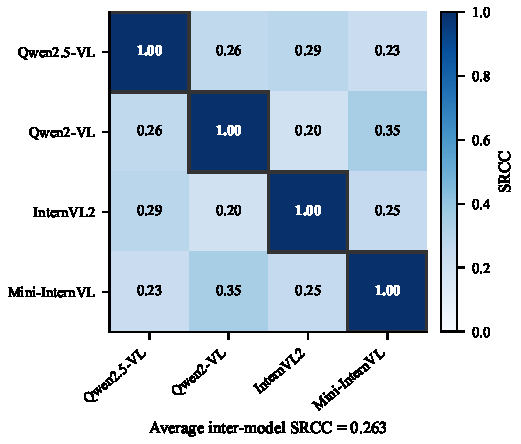
\includegraphics[width=0.45\textwidth]{figures/fig_vlm_corr.pdf}
    \caption{Spearman rank-order correlation (SRCC) between the four VLM annotators
    (Qwen2.5-VL, Qwen2-VL, InternVL2, Mini-InternVL) on the UAV-Embodied-IQA
    test set. The average off-diagonal SRCC is 0.26, consistent with Embodied-IQA's
    finding of $\sim$0.30 for VLM annotation of robot perception tasks.
    This low inter-model agreement motivates ensemble aggregation: using a
    single VLM as the sole annotation oracle is insufficient.}
    \label{fig:vlm_corr}
\end{figure}

% ── Figure: Dataset Statistics Overview (3-panel) ──
% Equivalent to AirCopBench Fig 3
\begin{figure*}[t]
    \centering
    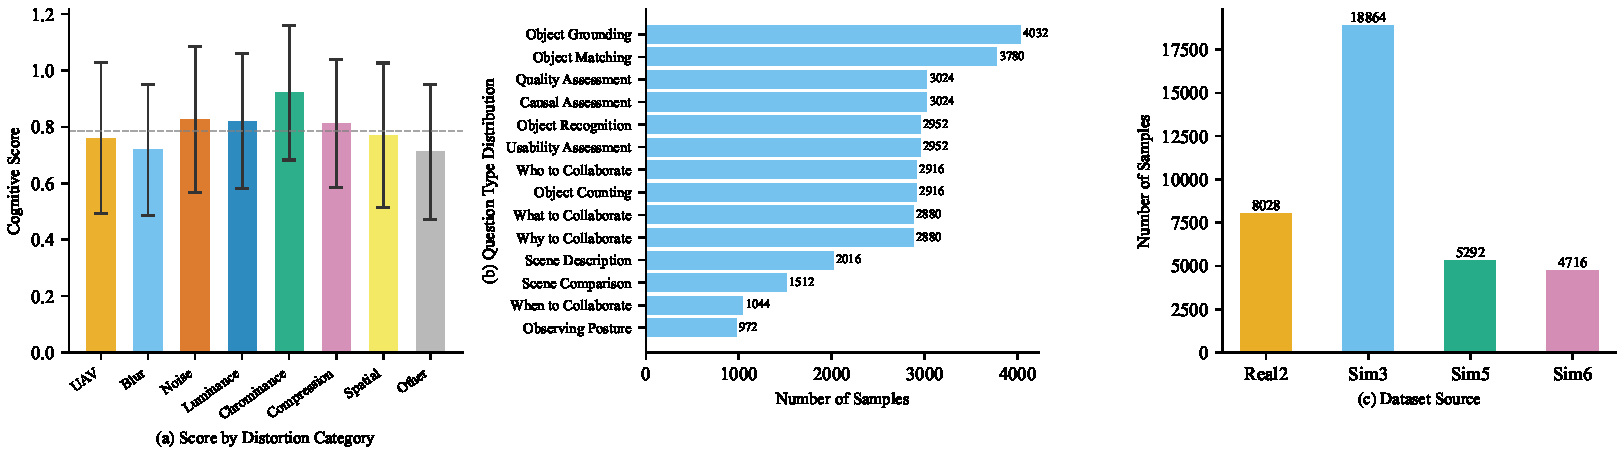
\includegraphics[width=\textwidth]{figures/fig_dataset_stats.pdf}
    \caption{UAV-Embodied-IQA database overview.
    (a) Cognitive score distribution by distortion category (box plots);
    UAV and Other categories have the widest spread.
    (b) Sample distribution across 14 question types; scene-description tasks
    dominate (11{,}736 samples), reflecting AirCopBench's task protocol.
    (c) Sample distribution across four data sources: Sim3 (AirCopBench,
    18{,}864), Real2 (MDMT real-world, 8{,}028), Sim5 (CARLA-Air, 5{,}292),
    Sim6 (MotionScape, 4{,}716).}
    \label{fig:dataset_stats}
\end{figure*}

% ── Table 1: Database Statistics ──
% \begin{table}[t]
\centering
\small
\setlength{\tabcolsep}{4pt}
\caption{UAV-Embodied-IQA database statistics. All splits (train + test). VLM annotations from 4 models: Qwen2.5-VL, Qwen2-VL, InternVL2, Mini-InternVL.}
\label{tab:db_stats}
\begin{tabular}{llccc}
\toprule
\textbf{Source} & \textbf{Type} & \textbf{Ref.\ Images} & \textbf{Dist.\ Types} & \textbf{Annotated Pairs} \\
\midrule
AirCopBench (Sim) & Sim & 609 & 36 & 305964 \\
CARLA-Air (Sim) & Sim & 47 & 36 & 36324 \\
MotionScape (Sim) & Sim & 49 & 36 & 70272 \\
MDMT (Real) & Real & 258 & 36 & 81792 \\
\midrule
\textbf{Total} & --- & \textbf{963} & \textbf{36} & \textbf{494352} \\
\bottomrule
\end{tabular}
\end{table}

% (or copy inline)

